%% Copyright (c) 2015-2019, RTE (http://www.rte-france.com)
%% See AUTHORS.txt
%% All rights reserved.
%% This Source Code Form is subject to the terms of the Mozilla Public
%% License, v. 2.0. If a copy of the MPL was not distributed with this
%% file, you can obtain one at http://mozilla.org/MPL/2.0/.
%% SPDX-License-Identifier: MPL-2.0
%%
%% This file is part of Dynawo, a hybrid C++/Modelica open source time domain simulation tool for power systems.

\documentclass[a4paper, 12pt]{report}

%% Except where otherwise noted, content in this documentation is Copyright (c)
%% 2015-2019, RTE (http://www.rte-france.com) and licensed under a
%% CC-BY-4.0 (https://creativecommons.org/licenses/by/4.0/)
%% license. All rights reserved.

% Latin Modern fam­ily of fonts
\usepackage{lmodern}

\usepackage[english]{babel}

% specify encoding
\usepackage[utf8]{inputenc} % input
\usepackage[T1]{fontenc} % output

% Document structure setup
\usepackage{titlesec} % To change chapter format
\setcounter{tocdepth}{3} % Add subsubsection in Content
\setcounter{secnumdepth}{3} % Add numbering for subsubsection
\setlength{\parindent}{0pt} % No paragraph indentation

% Change title format for chapter
\titleformat{\chapter}{\Huge\bf}{\thechapter}{20pt}{\Huge\bf}

% To add links on page number in Content and hide red rectangle on links
\usepackage[hidelinks, linktoc=all]{hyperref}
\usepackage[nottoc]{tocbibind}  % To add biblio in table of content
\usepackage{textcomp} % For single quote
\usepackage{url} % Allow linebreaks in \url command
\usepackage{listings} % To add code samples

% Default listings parameters
\lstset
{
  aboveskip={1\baselineskip}, % a bit of space above
  backgroundcolor=\color{shadecolor}, % choose the background color
  basicstyle={\ttfamily\footnotesize}, % use font and smaller size \small \footnotesize
  breakatwhitespace=true, % sets if automatic breaks should only happen at whitespace
  breaklines=true, % sets automatic line breaking
  columns=fixed, % nice spacing -> fixed / flexible
  mathescape=false, % escape to latex false
  numbers=left, % where to put the line-numbers
  numberstyle=\tiny\color{gray}, % the style that is used for the line-numbers
  showstringspaces=false, % do not emphasize spaces in strings
  tabsize=4, % number of spaces of a TAB
  texcl=false, % activates or deactivates LaTeX comment lines
  upquote=true % upright quotes
}

% Avoid numbering starting at each chapter for figures
\usepackage{chngcntr}
\counterwithout{figure}{chapter}

\usepackage{tikz} % macro pack­age for cre­at­ing graph­ics
\usepackage{pgfplots} % draws func­tion plots (based on pgf/tikz)

\usepackage{algorithm} % Add algorithms
\usepackage[noend]{algpseudocode} %  all end ... lines are omitted in algos

\usepackage{amsmath} % Add math­e­mat­i­cal fea­tures
\usepackage{schemabloc} % Add block diagram library (french one)

\usepackage{adjustbox} % Add box for flowchart

\usepackage{booktabs} % for toprule and midrule in tables

\usepackage{tabularx}

\usepackage[nolist]{acronym} % don’t write the list of acronyms.
% Acronyms list
\begin{acronym}
\acro{BDF}{Backward Differentiation Formula}
\acro{BE}{Backward Euler}
\acro{DAE}{Differential Algebraic Equations}
\acro{IDA}{Implicit Differential-Algebraic solver}
\acro{LLNL}{Lawrence Livermore National Lab}
\acro{KINSOL}{Krylov Inexact Newton SOLver}
\acro{NR}{Newton-Raphson}
\acro{PLL}{Phase-Locked Loop}
\acro{SVC}{Static Var Compensator}
\acro{SUNDIALS}{SUite of Nonlinear and DIfferential/ALgebraic equation Solvers}
\acro{WECC}{Western Electricity Coordinating Council}
\end{acronym}

% Syntax highlight
%% Except where otherwise noted, content in this documentation is Copyright (c)
%% 2015-2019, RTE (http://www.rte-france.com) and licensed under a
%% CC-BY-4.0 (https://creativecommons.org/licenses/by/4.0/)
%% license. All rights reserved.

\usepackage{color}

\definecolor{blue}{rgb}{0,0,1}
\definecolor{lightblue}{rgb}{.3,.5,1}
\definecolor{darkblue}{rgb}{0,0,.4}
\definecolor{red}{rgb}{1,0,0}
\definecolor{darkred}{rgb}{.56,0,0}
\definecolor{pink}{rgb}{.933,0,.933}
\definecolor{purple}{rgb}{0.58,0,0.82}
\definecolor{green}{rgb}{0.133,0.545,0.133}
\definecolor{darkgreen}{rgb}{0,.4,0}
\definecolor{gray}{rgb}{.3,.3,.3}
\definecolor{darkgray}{rgb}{.2,.2,.2}
\definecolor{shadecolor}{gray}{0.925}

% **********************************************************************************
% Syntax : Bash (bash)
% **********************************************************************************

\lstdefinelanguage{bash}
{
  keywordstyle=\color{blue},
  morekeywords={
    cd,
    export,
    source},
  numbers=none,
  deletekeywords={jobs}
}

% **********************************************************************************
% Syntax : XML
% **********************************************************************************

\lstdefinelanguage{XML}
{
  morestring=[s][\color{purple}]{"}{"},
  morecomment=[s][\color{green}]{<?}{?>},
  morecomment=[s][\color{green}]{<!--}{-->},
  stringstyle=\color{black},
  identifierstyle=\color{blue},
  keywordstyle=\color{red},
  morekeywords={
    xmlns,
    xsi,
    noNamespaceSchemaLocation,
    type,
    source,
    target,
    version,
    tool,
    transRef,
    roleRef,
    objective,
    eventually}
}

% **********************************************************************************
% Syntax : Modelica (modelica)
% **********************************************************************************
\lstdefinelanguage{Modelica}{
  alsoletter={...},
  morekeywords=[1]{ % types
      Boolean,
      Integer,
      Real},
  keywordstyle=[1]\color{red},
  morekeywords=[2]{ % keywords
    algorithm,
    and,
    annotation,
    assert,
    block,
    class,
    connector,
    constant,
    discrete,
    else,
    elseif,
    elsewhen,
    end,
    equation,
    exit,
    extends,
    external,
    false,
    final,
    flow,
    for,
    function,
    if,
    in,
    inner,
    input,
    import,
    loop,
    model,
    nondiscrete,
    not,
    or,
    outer,
    output,
    package,
    parameter,
    public,
    protected,
    record,
    redeclare,
    replaceable,
    return,
    size,
    terminate,
    then,
    true,
    type,
    when,
    while},
  keywordstyle=[2]\color{darkred},
  morekeywords=[3]{ % functions
    abs,
    acos,
    asin,
    atan,
    atan2,
    Complex,
    connect,
    conj,
    cos,
    cosh,
    cross,
    der,
    edge,
    exp,
    fromPolar,
    imag,
    noEvent,
    pre,
    sign,
    sin,
    sinh,
    sqrt,
    tan,
    tanh},
  keywordstyle=[3]\color{blue},
  morecomment=[l][\color{green}]{//}, % comments
  morecomment=[s][\color{green}]{/*}{*/}, % comments
  morestring=[b][\color{pink}]{'}, % strings
  morestring=[b][\color{pink}]{"}, % strings
}


\usepackage{xspace} % Define typography
\usepackage{dirtree}
\newcommand{\Dynawo}[0]{Dyna$\omega$o\xspace}


\begin{document}

\chapter{IEEE14 with Automata}

This document presents the different tests conducted on the IEEE 14-bus test case with the different automaton models that can be found in the \Dynawo library.\\

Here is the IEEE 14-bus system topology:
\begin{figure}[H]
  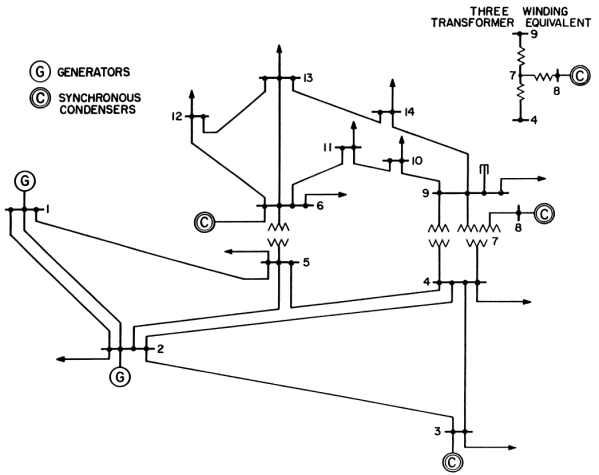
\includegraphics[width=\textwidth]{Single-line-diagram-of-IEEE-14-bus-system.png}
  \caption{IEEE 14 bus system diagram}
\end{figure}

The description of the data, models and other characteristics of the test case can be found in the IEEE14\_BasicTestSystems description directory. \\

For each test presented in this document, one or more automata have been added to the initial IEEE 14-bus test system introduced in the aforementioned description. All the modifications that have been made on this initial test case are listed and justified in the coming sections dedicated to the each automaton.\\

The tested automaton are;
\begin{itemize}
\item the under-voltage automaton [\ref{UnderVoltageAutomaton}];
\item the over-voltage automaton [\ref{OverVoltageAutomaton}];
\item the phase-shifter I automaton [\ref{PhaseShifterIAutomaton}];
\item the phase-shifter P automaton [\ref{PhaseShifterPAutomaton}];
\item the current limit automaton [\ref{CurrentLimitAutomaton}];
\item the tap-changer automaton (Modelica) [\ref{TapChangerAutomatonModelica}];
\item the tap-changer automaton (C++) [\ref{TapChangerAutomatonCpp}];
\item the tap-changer blocking automaton [\ref{TapChangerBlockingAutomaton}];
\item the line distance protection [\ref{DistanceProtection}];
\item the loss-of-synchronism-protection [\ref{LossOfSynchronismProtection}];
\item the over- and under-speed protection [\ref{SpeedProtection}];
\item the under-frequency load shedding scheme [\ref{UFLS}];
\end{itemize}


\newpage
\section{Under voltage automaton}
\label{UnderVoltageAutomaton}

The under voltage automaton disconnects a generator from the grid if its voltage is under a certain threshold for a certain amount of time.

\subsection{Initial Conditions}

Initial conditions are the same that in the IEEE 14-bus basic test cases.

\subsection{Models}

An under voltage automaton is added on the generator number 3. The role of the automaton is to disconnect the generator if its voltage drops too much. The generators regulations are removed for this test in order to simulate a deep voltage drop that can activate the under voltage automaton.\\

The under voltage automaton measures the generator voltage (in this test at its network connection point) and sends the disconnection order when the voltage has spent more than $t_{Action}$ seconds under $U_{Min}$.\\

The under voltage automaton parameters are:
\begin{center}
\begin{tabular}{l|l}
   $U_{Min_{Pu}}=0.85pu$ & $t_{Action}=5s$  \\
\end{tabular}
\end{center}

\subsection{Scenario}
At $t=20s$, the following load variations are simulated:
\begin{itemize}
\item{the active and reactive power of load 2 are changed from $P=21.7MW$ and $Q=12.7Mvar$ to $P=100MW$ and $Q=200Mvar$}
\item{the active and reactive power of load 3 are changed from $P=94.2MW$ and $Q=19Mvar$ to $P=200MW$ and $Q=200Mvar$}
\end{itemize}

\subsection{Solver}
The solver used is the variable time step solver IDA with the following parameters:
\begin{center}
\begin{tabular}{l|l|l}
   $Order$=2 & $Accuracy_{Rel}$=10e-4 & $Accuracy_{Abs}$=10e-4 \\
\end{tabular}
\end{center}

\newpage
\subsection{Results}

The simulated load variations make the network voltage decrease at node 3, until achieving the minimum threshold of the automaton. The generator is disconnected 5 seconds later, which corresponds to the action time.\\

\begin{figure}[H]
\subfigure[Generator 3 stator voltage (pu)]
{%
  \begin{tikzpicture}
    \begin{axis}[height = 2in]
        \addplot[color=blue!50]
        table[x=time, y expr=\thisrow{NETWORK__BUS____3_TN_Upu_value}]
        {../IEEE14_UnderVoltageAutomaton/reference/outputs/curves/curves.csv};
        \addplot[color=red!50]
        table[x=time, y expr=\thisrow{UVA_underVoltageAutomaton_UMinPu}]
        {../IEEE14_UnderVoltageAutomaton/reference/outputs/curves/curves.csv};
        \legend{$U_{Stator_{Pu}}$, $U_{Min_{Pu}}$}
    \end{axis}
  \end{tikzpicture}
}
\subfigure[Generator 3 running status]
{%
  \begin{tikzpicture}
    \begin{axis}[height = 2in]
        \addplot[color=blue!50]
        table[x=time, y expr=\thisrow{GEN____3_SM_generator_running}]
        {../IEEE14_UnderVoltageAutomaton/reference/outputs/curves/curves.csv};
    \end{axis}
  \end{tikzpicture}
}
\caption{Behavior of the under voltage automaton}
\end{figure}


\newpage
\section{Over voltage automaton}
\label{OverVoltageAutomaton}

The over voltage automaton disconnects a generator from the grid if its voltage is above a certain threshold for a certain amount of time.

\subsection{Initial Conditions}

Initial conditions are the same that in the IEEE 14-bus basic test cases.

\subsection{Models}

An over voltage automaton is added on the generator number 3. The role of the automaton is to disconnect the generator if its voltage gets higher than the threshold.
Also an under voltage automaton is added in this model to test if there are any undesired interactions between the two protections. The generators regulations are removed for this test case.\\

The over voltage automaton measures the generator voltage (in this test at its network connection point) and sends the disconnection order when the voltage has spent more than $t_{Action}$ seconds above $U_{Max}$.\\

The over voltage automaton parameters are:
\begin{center}
\begin{tabular}{l|l}
   $U_{Max_{Pu}}= 1.05\ pu$ & $t_{Action}=5s$  \\
\end{tabular}
\end{center}

\subsection{Scenario}
At $t=20s$, the following load variations are simulated:
\begin{itemize}
\item{the reactive power of load 2 is changed from $Q=12.7\ Mvar$ to $Q=-37.3\ Mvar$}
\item{the reactive power of load 3 is changed from $Q=19\ Mvar$ to $Q=-31\ Mvar$}
\end{itemize}

\subsection{Solver}
The solver used is the variable time step solver IDA with the following parameters:
\begin{center}
\begin{tabular}{l|l|l}
   $Order$=2 & $Accuracy_{Rel}$=10e-4 & $Accuracy_{Abs}$=10e-4 \\
\end{tabular}
\end{center}

\newpage
\subsection{Results}

The simulated load variations make the network voltage increase at node 3, until achieving the maximum threshold of the automaton. The generator is disconnected 5 seconds later, which corresponds to the action time.\\

\begin{figure}[H]
\subfigure[Generator 3 stator voltage (pu)]
{%
  \begin{tikzpicture}
    \begin{axis}[height = 2in]
        \addplot[color=blue!50]
        table[x=time, y expr=\thisrow{NETWORK__BUS____3_TN_Upu_value}]
        {../IEEE14_OverVoltageAutomaton/reference/outputs/curves/curves.csv};
        \addplot[color=red!50]
        table[x=time, y expr=\thisrow{OVA_overVoltageAutomaton_UMaxPu}]
        {../IEEE14_OverVoltageAutomaton/reference/outputs/curves/curves.csv};
        \legend{$U_{Stator_{Pu}}$, $U_{Max_{Pu}}$}
    \end{axis}
  \end{tikzpicture}
}
\subfigure[Generator 3 running status]
{%
  \begin{tikzpicture}
    \begin{axis}[height = 2in]
        \addplot[color=blue!50]
        table[x=time, y expr=\thisrow{GEN____3_SM_generator_running}]
        {../IEEE14_OverVoltageAutomaton/reference/outputs/curves/curves.csv};
    \end{axis}
  \end{tikzpicture}
}
\caption{Behavior of the over voltage automaton}
\end{figure}

\newpage
\section{Phase Shifter I}
\label{PhaseShifterIAutomaton}

The phase-shifter I is an automaton that gradually changes the tap of a phase-shifter transformer if its monitored transiting current goes higher than a defined threshold for a certain amount of time.

\subsection{Initial Conditions}

Initial conditions are the same that in the IEEE 14-bus basic test cases.

\subsection{Models}

Instead of a ratio tap changer transformer (no phase shift) between buses 5 and 6, we use a phase tap changer transformer controlled by a phase-shifter I automaton in order to regulate the transiting current.
The automaton is supposed to keep the transit under a given threshold, by reducing or increasing the phase shift step by step. \\

The phase-shifter I measures the current flowing through a transformer and sends an order to change its tap if the monitored transiting current stays higher than $I_{Max}$ for a certain amount of time. Then the automaton keeps on making the transformer change its tap until its current reaches $I_{Stop}$. The first tap is changed after a delay $t_{1st}$ and the next taps are changed after $t_{Next}$ seconds. \\

The phase-shifter parameters are:
\begin{center}
\begin{tabular}{l|l|l}
   $I_{Max}=0.475pu$ & $t_{1st}=10s$ & $tap_{Max}=13$ \\
   $I_{Stop}=0.45pu$  & $t_{Next}=5s$ & $tap_{Min}=1$ \\
\end{tabular}
\end{center}

\subsection{Scenario}
At $t=20s$, the following line disconnection is simulated:
\begin{itemize}
\item{the line connecting bus 9 to bus 10 is opened at its bus 10 end}
\end{itemize}

\subsection{Solver}
The solver used is the variable time step solver IDA with the following parameters:
\begin{center}
\begin{tabular}{l|l|l}
   $Order$=2 & $Accuracy_{Rel}$=10e-4 & $Accuracy_{Abs}$=10e-4 \\
\end{tabular}
\end{center}

\newpage
\subsection{Results}

At t=20s, the line is disconnected. Following the topology modification, the current through the transformer monitored by the phase shifter I becomes higher than its threshold $I_{Max}$. After a time delay of 10s, the phase shifter changes its first step, which results in a step decrease of the transformer's current. Then, step are changed every 5s and the process repeats until the current reaches $I_{Stop}$ and don't cross $I_{Max}$ again. \\

\begin{figure}[H]
\subfigure[Transformer's current (pu)]
{%
  \begin{tikzpicture}
    \begin{axis}[height = 2in]
        \addplot[dashed, color=red!50]
        table[dashed, x=time,y=PhaseShifter_phaseShifter_iMax]
        {../IEEE14_PhaseShifterI/reference/outputs/curves/curves.csv};
        \addplot[color=blue!50]
        table[x=time,y=PhaseShifter_phaseShifter_iMonitored]
        {../IEEE14_PhaseShifterI/reference/outputs/curves/curves.csv};
        \addplot[dashed, color=green!50]
        table[x=time,y=PhaseShifter_phaseShifter_iStop]
        {../IEEE14_PhaseShifterI/reference/outputs/curves/curves.csv};
        \legend{$I_{Max_{Pu}}$, $I_{Pu}$, $I_{Stop_{Pu}}$}
    \end{axis}
  \end{tikzpicture}
}
\subfigure[Transformer's tap]
{%
\begin{tikzpicture}
    \begin{axis}[height = 2in]
        \addplot[color=blue!50]
        table[x=time,y=NETWORK__BUS____5-BUS____6-1_PS_step]
        {../IEEE14_PhaseShifterI/reference/outputs/curves/curves.csv};
        \legend{$Tap$}
    \end{axis}
  \end{tikzpicture}
}
\caption{Behavior of the phase-shifter I}
\end{figure}


\newpage
\section{Phase Shifter P}
\label{PhaseShifterPAutomaton}

The phase-shifter P is an automaton that gradually changes the tap of a phase-shifter transformer if its monitored transiting active power goes out of a certain range for a certain amount of time.

\subsection{Initial Conditions}

Initial conditions are the same that in the IEEE 14-bus basic test cases.

\subsection{Models}

Instead of a ratio tap changer transformer (no phase shift) between buses 5 and 6, we use a phase tap changer transformer controlled by a phase-shifter P automaton in order to regulate the transiting active power.
The automaton is supposed to keep the transit within acceptable bounds, by reducing or increasing the phase shift step by step. \\

The phase-shifter P measures the transiting active power through a transformer and sends an order to change the its tap if the monitored active power differs from $P_{target}$ by more than $P_{DeadBand}$. The first tap is changed after the time $t_{1st}$ and the next taps are changed after $t_{Next}$ seconds.\\

The phase-shifter parameters are:
\begin{center}
\begin{tabular}{l|l|l}
   $P_{target}=0.44pu$ & $t_{1st}=10s$ & $tap_{Max}=13$ \\
   $P_{DeadBand}=0.005pu$  & $t_{Next}=5s$ & $tap_{Min}=1$ \\
\end{tabular}
\end{center}

\subsection{Scenario}
At $t=20s$, the following line disconnection is simulated:
\begin{itemize}
\item{the line connecting bus 9 to bus 10 is opened at its bus 10 end}
\end{itemize}

\subsection{Solver}
The solver used is the variable time step solver IDA with the following parameters:
\begin{center}
\begin{tabular}{l|l|l}
   $Order$=2 & $Accuracy_{Rel}$=10e-4 & $Accuracy_{Abs}$=10e-4 \\
\end{tabular}
\end{center}

\newpage
\subsection{Results}

At t=20s, the line is disconnected. Following the topology modification, the current through the transformer monitored by the phase shifter goes out of the tolerated range around $P_{Target}$.  10 seconds later, the transformer tap is changed which results in a step decrease of transiting active power. Though, it is still not in the tolerated range so the phase-shifter increases the tap again, this time only waiting for 5 seconds. Consequently, the active power transit drops and transiently falls back into the dead-band before going out of it again. Therefore, the phase-shifter P first temporarily stops taking steps, and then starts again waiting for a 10s delay before shifting to the next tap. This process repeats two times more and the automaton stops acting once the active power transit finally stabilizes in the range around $P_{Target}$. \\

\begin{figure}[H]
\subfigure[Transformer's transiting active power (pu)]
{%
  \begin{tikzpicture}
    \begin{axis}[height = 2in]
        \addplot[dashed, color=red!50]
        table[x=time, y=PhaseShifter_phaseShifter_valueMax]
        {../IEEE14_PhaseShifterP/reference/outputs/curves/curves.csv};
        \addplot[color=blue!50]
        table[x=time, y=PhaseShifter_phaseShifter_PMonitored]
        {../IEEE14_PhaseShifterP/reference/outputs/curves/curves.csv};
        \addplot[dashed, color=green!50]
        table[x=time, y=PhaseShifter_phaseShifter_valueMin]
        {../IEEE14_PhaseShifterP/reference/outputs/curves/curves.csv};
        \legend{$P_{Max_{Pu}}$, $P_{Pu}$, $P_{Min_{Pu}}$}
    \end{axis}
  \end{tikzpicture}
}
\subfigure[Transformer's tap]
{%
\begin{tikzpicture}
    \begin{axis}[height = 2in]
        \addplot[color=blue!50]
        table[x=time,y=NETWORK__BUS____5-BUS____6-1_PS_step]
        {../IEEE14_PhaseShifterP/reference/outputs/curves/curves.csv};
        \legend{$Tap$}
    \end{axis}
  \end{tikzpicture}
}
\caption{Behavior of the phase-shifter P}
\end{figure}


\newpage
\section{Current limit automaton}
\label{CurrentLimitAutomaton}

The current limit automaton monitors a line's transiting current and opens it if it is superior to a defined threshold for a certain amount of time.

\subsection{Initial Conditions}

Initial conditions are the same that in the IEEE 14-bus basic test cases.

\subsection{Models}

Two current limit automata are added to the network : one monitoring the line connecting bus 2 to bus 4, one monitoring the line connecting bus 2 to bus 5.
Automata's role is to protect their line from unbearable currents by disconnecting it after a too long over-current constraint. \\

The current limit automaton measures the current transiting through a line and sends an order to disconnect it if it stays more than $t_{Action}$ seconds above the threshold $I_{Max}$. The order also specifies the type of disconnection (origin end, extremity end, or both).\\

The current limit automaton monitoring line bus2-bus5 parameters are:
\begin{center}
\begin{tabular}{l|l|l}
   $I_{Max}=600A$ & $t_{Action}=5$ & $order=1$ (disconnect both ends)\\
\end{tabular}
\end{center}

The current limit automaton monitoring line bus2-bus4 parameters are:
\begin{center}
\begin{tabular}{l|l|l}
   $I_{Max}=1000A$ & $t_{Action}=10$ & $order=3$ (disconnect bus 4 end)\\
\end{tabular}
\end{center}

\subsection{Scenario}
At $t=5s$, the following line disconnection is simulated:
\begin{itemize}
\item{the line connecting bus 1 to bus 5 is opened at its bus 5 end}
\end{itemize}

\subsection{Solver}
The solver used is the variable time step solver IDA with the following parameters:
\begin{center}
\begin{tabular}{l|l|l}
   $Order$=2 & $Accuracy_{Rel}$=10e-4 & $Accuracy_{Abs}$=10e-4 \\
\end{tabular}
\end{center}


\newpage
\subsection{Results}

At t=5s, the line 1-5 is disconnected. Following this topology change, the current value on the line 2-5 monitored by the first current limit automaton becomes higher than its threshold $I_{Max}$=600 A. After the time delay (5s), and as the current didn't go back under $I_{Max}$, the automaton then opens line 2-5.
As a consequence, the transit on line 2-4 increases and exceeds the second current limit automaton threshold $I_{Max}$=1000 A . After the time delay (10s), and as the current didn't go back under $I_{Max}$, the automaton opens line 2-4. \\

\begin{figure}[H]
\subfigure[Currents monitored by the automata (A)]
{%
  \begin{tikzpicture}
    \begin{axis}[height = 2in]
        \addplot[color=green!50]
        table[x=time,y=NETWORK__BUS____2-BUS____5-1_AC_iSide2]
        {../IEEE14_CurrentLimitAutomaton/reference/outputs/curves/curves.csv};
        \addplot[color=blue!50]
        table[x=time,y=NETWORK__BUS____2-BUS____4-1_AC_iSide2]
        {../IEEE14_CurrentLimitAutomaton/reference/outputs/curves/curves.csv};
        \addplot[dashed, color=red!50]
        table[x=time,y=CLA_2_4_currentLimitAutomaton_IMax]
        {../IEEE14_CurrentLimitAutomaton/reference/outputs/curves/curves.csv};
        \addplot[dashed, color=orange!50]
        table[x=time,y=CLA_2_5_currentLimitAutomaton_IMax]
        {../IEEE14_CurrentLimitAutomaton/reference/outputs/curves/curves.csv};
        \legend{$I_{bus2\_bus5}$, $I_{bus2\_bus4}$, $I_{Max_{CLA\_2\_4}}$, $I_{Max_{CLA\_2\_5}}$}
    \end{axis}
  \end{tikzpicture}
}
\subfigure[Automata's orders sent to the lines]
{%
  \begin{tikzpicture}
    \begin{axis}[legend pos=south east, height = 2in]
        \addplot[color=blue!50]
        table[x=time,y=CLA_2_5_currentLimitAutomaton_order]
        {../IEEE14_CurrentLimitAutomaton/reference/outputs/curves/curves.csv};
        \addplot[color=red!50]
        table[x=time,y=CLA_2_4_currentLimitAutomaton_order]
        {../IEEE14_CurrentLimitAutomaton/reference/outputs/curves/curves.csv};
        \legend{$Order_{CLA\_2\_5}$, $Order_{CLA\_2\_4}$}
    \end{axis}
  \end{tikzpicture}
}
\caption{Behavior of the current limit automata}
\end{figure}

\newpage
\section{Tap Changer (Modelica)}
\label{TapChangerAutomatonModelica}

The tap-changer is an automaton that changes the tap of a transformer if its monitored terminal voltage goes out of a certain range for a certain amount of time. In this test, the Modelica model is tested.

\subsection{Initial Conditions}

Initial conditions are the same that in the IEEE 14-bus basic test cases.

\subsection{Models}

Load number 3 is moved behind a transformer equipped with a tap-changer. The role of the tap-changer is to maintain the load terminal voltage within a certain range, independently of what happens on the transmission system level. \\

The tap-changer measures the load terminal voltage and sends an order to change the transformer tap if the monitored voltage differs from $U_{target}$ by more than $U_{DeadBand}$. The first tap is changed after the time $t_{1st}$ and the next taps are changed after $t_{Next}$ seconds.\\

The tap-changer parameters are:
\begin{center}
\begin{tabular}{l|l|l}
   $U_{Target}=1pu$ & $t_{1st}=60s$ & $tap_{Max}=84$ \\
   $U_{DeadBand}=0.01pu$  & $t_{Next}=10s$ & $tap_{Min}=0$ \\
\end{tabular}
\end{center}

\subsection{Scenario}
At $t=20s$, the following load variation is simulated:
\begin{itemize}
\item{the reactive power of load 3 is changed from $Q=12.7Mvar$ to $Q=30Mvar$}
\end{itemize}

\subsection{Solver}
The solver used is the variable time step solver IDA with the following parameters:
\begin{center}
\begin{tabular}{l|l|l}
   $Order$=2 & $Accuracy_{Rel}$=10e-4 & $Accuracy_{Abs}$=10e-4 \\
\end{tabular}
\end{center}

\newpage
\subsection{Results}

The simulated load variation makes the network voltage drop at node 3. The load 3 terminal voltage also decreases until it goes out of the tolerated range around $U_{Target}$. 60 seconds later, the transformer tap is changed which results in a step increase of the load terminal voltage. The voltage is still not in the tolerated range so the tap-changer changes the tap again, this time only waiting for 10 seconds, and stops acting once the load terminal voltage finally reaches the range around $U_{Target}$.

\begin{figure}[H]
\subfigure[Load terminal voltage (pu)]
{%
  \begin{tikzpicture}
    \begin{axis}[height = 2.5in, yticklabel style={text width={width("$-0.6$")},align=right}]
        \addplot[color=red!50]
        table[x=time, y expr=\thisrow{TAP_CHANGER_LOAD_3_tapChanger_valueMax}]
        {../IEEE14_TapChanger/reference/outputs/curves/curves.csv};
        \addplot[color=blue!50]
        table[x=time, y expr=\thisrow{_LOAD___3_EC_transformer_U2Pu}]
        {../IEEE14_TapChanger/reference/outputs/curves/curves.csv};
        \addplot[color=green!50]
        table[x=time, y expr=\thisrow{TAP_CHANGER_LOAD_3_tapChanger_valueMin}]
        {../IEEE14_TapChanger/reference/outputs/curves/curves.csv};
        \legend{$U_{Max_{Pu}}$, $U_{Pu}$, $U_{Min_{Pu}}$}
    \end{axis}
  \end{tikzpicture}
}
\subfigure[Transformer tap]
{%
  \begin{tikzpicture}
    \begin{axis}[height = 2in, yticklabel style={text width={width("$-0.6$")},align=right}]
        \addplot[color=blue!50]
        table[x=time, y expr=\thisrow{_LOAD___3_EC_transformer_tap}]
        {../IEEE14_TapChanger/reference/outputs/curves/curves.csv};
    \end{axis}
  \end{tikzpicture}
}
\caption{Behavior of the tap-changer}
\end{figure}

\begin{figure}[H]
\subfigure[Network voltage at bus 3 (pu)]
{%
  \begin{tikzpicture}
    \begin{axis}[height = 2.5in]
        \addplot[color=blue!50]
        table[x=time, y expr=\thisrow{NETWORK__BUS____3_TN_Upu_value}]
        {../IEEE14_TapChanger/reference/outputs/curves/curves.csv};
    \end{axis}
  \end{tikzpicture}
}
\caption{Impact of the transformer tap modification on the network voltage}
\end{figure}

We observe that changing the tap helps restoring the load terminal voltage but has a negative impact on the network voltage: each time the tap is increased, the network voltage is decreased a little. If many transformers are changing taps at the same time and on the same network area it could lead to a general voltage collapse. In order to avoid this phenomena, other automata called "Tap-Changer Block" monitor the network voltage and can stop the transformers from changing their taps.


\newpage
\section{Tap Changer (CPP)}
\label{TapChangerAutomatonCpp}

The tap-changer is an automaton that changes the tap of a transformer if its monitored terminal voltage goes out of a certain range for a certain amount of time. In this test, the default C++ model is tested.

\subsection{Initial Conditions}

Initial conditions are the same that in the IEEE 14-bus basic test cases.

\subsection{Models}

Transformer 5-6 tap-changer has been activated to control the voltage at the transformer higher terminal (node 5). The role of the tap-changer is to maintain the high terminal voltage within a certain range, independently of what happens on the other terminal. \\

The tap-changer measures the high terminal voltage and sends an order to change the transformer tap if the monitored voltage differs from $targetV$ by more than $tolV$. The first tap is changed after the time $t1st_{HT}$ and the next taps are changed after $tNext_{HT}$ seconds.\\

The tap-changer parameters are:
\begin{center}
\begin{tabular}{l|l}
   $targetV=1pu$ & $t1st_{HT}=60s$ \\
   $tolV=0.01pu$  & $tNext_{HT}=10s$ \\
\end{tabular}
\end{center}

Note: As we use the default C++ ratio tap-changer model, no information is added in the .dyd file, but rather in the .iidm file. The sequence "terminalRef" should be added with the attributes $id$ and $side$, and the target voltage $targetV$ should be given as attribute of the "ratioTapChanger". All the other parameters are given in the .par file, in the network parameters set.

\subsection{Scenario}
At $t=20s$, the following load variation is simulated:
\begin{itemize}
\item{the reactive power of load 5 is changed from $Q=1.6Mvar$ to $Q=84Mvar$}
\end{itemize}

\subsection{Solver}
The solver used is the variable time step solver IDA with the following parameters:
\begin{center}
\begin{tabular}{l|l|l}
   $Order$=2 & $Accuracy_{Rel}$=10e-4 & $Accuracy_{Abs}$=10e-4 \\
\end{tabular}
\end{center}

\subsection{Results}

The simulated load variation makes the network voltage drop at node 5, going out of the tolerated range around $targetV$. 60 seconds later, the transformer tap is changed which results in a step increase of the node 5 voltage. The voltage is still not in the tolerated range so the tap-changer changes the tap again, this time only waiting for 10 seconds, and stops acting once the voltage finally reaches the range around $targetV$.

\begin{figure}[H]
\subfigure[Load terminal voltage (pu)]
{%
  \begin{tikzpicture}
    \begin{axis}[height = 2.5in, yticklabel style={text width={width("$-0.6$")},align=right}]
        \addplot[color=red!50]
        table[x=time, y expr=\thisrow{NETWORK__BUS____5_TN_Upu_value}]
        {../IEEE14_TapChangerCpp/reference/outputs/curves/curves.csv};
        \addplot[color=blue!50]
        table[x=time, y expr=\thisrow{NETWORK__BUS____6_TN_Upu_value}]
        {../IEEE14_TapChangerCpp/reference/outputs/curves/curves.csv};
        \legend{$U_{Node5}$, $U_{Node6}$}
    \end{axis}
  \end{tikzpicture}
}
\subfigure[Transformer tap]
{%
  \begin{tikzpicture}
    \begin{axis}[height = 1.7in, yticklabel style={text width={width("$-0.6$")},align=right}]
        \addplot[color=blue!50]
        table[x=time, y expr=\thisrow{NETWORK__BUS____5-BUS____6-1_PT_step}]
        {../IEEE14_TapChangerCpp/reference/outputs/curves/curves.csv};
    \end{axis}
  \end{tikzpicture}
}
\caption{Behavior of the tap-changer}
\end{figure}

\newpage
\section{Tap Changer Lock}
\label{TapChangerBlockingAutomaton}

The tap-changer lock automaton is an automaton that can prevent the tap-changers of a given area to change the tap of their transformers if the area monitored voltage  goes under a certain threshold for a certain amount of time. This automaton should prevent the network to experience voltage collapses.

\subsection{Initial Conditions}

Initial conditions are the same that in the IEEE 14-bus basic test cases.

\subsection{Models}

Load number 2 and 3 are moved behind a transformer equipped with a tap-changer. A tap-changer lock automaton which observes the voltage at the bus number 3 is added to the test case. It can lock the tap-changers of the aforementioned loads. \\

The tap-changer lock automaton activates a lock order if the monitored voltage goes under $U_{Min}$ for $t_{BeforeLocked}$ seconds. The lock order is then send to the tap-changer in $t_{TransLockedT}$ seconds for a load behind one transformer. For a load behind two transformers this time lag $t_{TransLockedT}$ corresponds to the sending time of the order to the transmission transformer and $t_{TransLockedD}$ corresponds to the sending time of the order to the distribution transformer. \\

The tap-changer lock automaton parameters are:
\begin{center}
\begin{tabular}{l|l}
   $U_{Min}=0.9824pu$ & $t_{TransLockedT}=10s$ \\
   $t_{BeforeLocked}=20s$  & $t_{TransLockedD}=10s$ \\
\end{tabular}
\end{center}

\subsection{Scenario}
At $t=20s$, the following load variations are simulated:
\begin{itemize}
\item{the reactive power of load 2 is changed from $Q=12.08Mvar$ to $Q=200Mvar$}
\item{the reactive power of load 3 is changed from $Q=12.7Mvar$ to $Q=200Mvar$}
\end{itemize}

\subsection{Solver}
The solver used is the variable time step solver IDA with the following parameters:
\begin{center}
\begin{tabular}{l|l|l}
   $Order$=2 & $Accuracy_{Rel}$=10e-4 & $Accuracy_{Abs}$=10e-4 \\
\end{tabular}
\end{center}

\subsection{Results}

The simulated load variations make the network voltage drop at node 2 and 3 (monitored by the tap-changer lock automaton), as well as the load terminal voltages (monitored by the loads transformers tap-changers). From $t=80s$ to $t=120s$, the load 2 and 3 tap-changers change the transformers taps to restore the voltage at the load terminal, which damages the network voltage.

\begin{figure}[H]
\subfigure[Load 2 and 3 terminal voltages (pu)]
{%
  \begin{tikzpicture}
    \begin{axis}[height = 2.3in]
        \addplot[color=blue!50]
        table[x=time, y expr=\thisrow{_LOAD___2_EC_transformer_U2Pu}]
        {../IEEE14_TapChangerBlocking/reference/outputs/curves/curves.csv};
        \addplot[color=red!50]
        table[x=time, y expr=\thisrow{_LOAD___3_EC_transformer_U2Pu}]
        {../IEEE14_TapChangerBlocking/reference/outputs/curves/curves.csv};
        \legend{$U_{Load2}$, $U_{Load3}$}
    \end{axis}
  \end{tikzpicture}
}
\subfigure[Network voltage at bus 2 and 3 (pu)]
{%
  \begin{tikzpicture}
    \begin{axis}[height = 2.3in]
        \addplot[color=blue!50]
        table[x=time, y expr=\thisrow{NETWORK__BUS____2_TN_Upu_value}]
        {../IEEE14_TapChangerBlocking/reference/outputs/curves/curves.csv};
        \addplot[color=green!50]
        table[x=time, y expr=\thisrow{NETWORK__BUS____3_TN_Upu_value}]
        {../IEEE14_TapChangerBlocking/reference/outputs/curves/curves.csv};
        \legend{$U_{Node2}$, $U_{Node3}$}
    \end{axis}
  \end{tikzpicture}
}
\caption{Voltages at the loads transformers primary and secondary sides}
\end{figure}

At $t=100s$,the tap-changer lock automaton monitored voltage crosses $U_{Min}$ permanently. The lock order of the tap-changer lock automaton is activated 20 seconds after that, and received by the load transformer 10 seconds later. The load transformers then stop to change taps and the network voltage stops decreasing.

\begin{figure}[H]
\subfigure[Tap-Changer Lock automaton monitored voltage (kV)]
{%
  \begin{tikzpicture}
    \begin{axis}[height = 2.7in]
        \addplot[color=blue!50]
        table[x=time, y expr=\thisrow{NETWORK__BUS____3_TN_U_value}]
        {../IEEE14_TapChangerBlocking/reference/outputs/curves/curves.csv};
        \addplot[color=red!50]
        table[x=time, y expr=\thisrow{TAP_CHANGER_LOCK_tapChangerBlocking_UMin}]
        {../IEEE14_TapChangerBlocking/reference/outputs/curves/curves.csv};
        \legend{$U_{Node3}$, $U_{Min}$}
    \end{axis}
  \end{tikzpicture}
}
\subfigure[Tap-Changer Lock automaton lock order]
{%
  \begin{tikzpicture}
    \begin{axis}[height = 1.5in, legend pos=north west]
        \addplot[color=red!50]
        table[x=time, y expr=\thisrow{TAP_CHANGER_LOCK_tapChangerBlocking_state}]
        {../IEEE14_TapChangerBlocking/reference/outputs/curves/curves.csv};
        \addplot[color=blue!50]
        table[x=time, y expr=\thisrow{TAP_CHANGER_LOCK_tapChangerBlocking_blockedD}]
        {../IEEE14_TapChangerBlocking/reference/outputs/curves/curves.csv};
        \addplot[dashed, color=green!50]
        table[x=time, y expr=\thisrow{TAP_CHANGER_LOCK_tapChangerBlocking_blockedT}]
        {../IEEE14_TapChangerBlocking/reference/outputs/curves/curves.csv};
        \legend{$state$, $LockedD$, $LockedT$}
    \end{axis}
  \end{tikzpicture}
}
\subfigure[Load 2 and 3 transformers taps]
{%
  \begin{tikzpicture}
    \begin{axis}[height = 1.5in, legend pos=north west]
        \addplot[color=blue!50]
        table[x=time, y expr=\thisrow{_LOAD___2_EC_transformer_tap}]
        {../IEEE14_TapChangerBlocking/reference/outputs/curves/curves.csv};
        \addplot[color=red!50]
        table[x=time, y expr=\thisrow{_LOAD___3_EC_transformer_tap}]
        {../IEEE14_TapChangerBlocking/reference/outputs/curves/curves.csv};
        \legend{$Tap_{Load2}$, $Tap_{Load3}$}
    \end{axis}
  \end{tikzpicture}
}
\caption{Behaviour of the Tap-Changer Lock automaton}
\end{figure}

If we try to simulate this test case without the tap-changer lock automaton we see that the transformers of load 2 and 3 keep changing taps and that the voltages of the area keep decreasing. In order to run this scenario, two possibilities are available: delete the tap-changer lock automaton in the .dyd file (with its connections), or set the automaton threshold $UMin=0$ in the .par file (that way the automaton will never get activated).

\begin{figure}[H]
\subfigure[Network voltage at bus 2 and 3 (pu)]
{%
  \begin{tikzpicture}
    \begin{axis}[height = 2.5in]
        \addplot[color=blue!50]
        table[x=time, y expr=\thisrow{NETWORK__BUS____2_TN_Upu_value}]
        {../IEEE14_TapChangerBlocking/referenceNoTCL/outputs/curves/curves.csv};
        \addplot[color=green!50]
        table[x=time, y expr=\thisrow{NETWORK__BUS____3_TN_Upu_value}]
        {../IEEE14_TapChangerBlocking/referenceNoTCL/outputs/curves/curves.csv};
        \legend{$U_{Node2}$, $U_{Node3}$}
    \end{axis}
  \end{tikzpicture}
}
\subfigure[Load 2 and 3 transformers taps]
{%
  \begin{tikzpicture}
    \begin{axis}[height = 2in, legend pos=north west]
        \addplot[color=blue!50]
        table[x=time, y expr=\thisrow{_LOAD___2_EC_transformer_tap}]
        {../IEEE14_TapChangerBlocking/referenceNoTCL/outputs/curves/curves.csv};
        \addplot[color=red!50]
        table[x=time, y expr=\thisrow{_LOAD___3_EC_transformer_tap}]
        {../IEEE14_TapChangerBlocking/referenceNoTCL/outputs/curves/curves.csv};
        \legend{$Tap_{Load2}$, $Tap_{Load3}$}
    \end{axis}
  \end{tikzpicture}
}
\caption{Results with no Tap-Changer Lock automaton}
\end{figure}

\newpage
\section{Line distance protection}
\label{DistanceProtection}

The line distance protection disconnects a line from the grid if the apparent impedance seen from a given end of the line is within a triangular zone in the R-X place for a certain amount of time.

\subsection{Initial Conditions}

Initial conditions are the same that in the IEEE 14-bus basic test cases.

\subsection{Models}

A distance protection is added on the side 1 of line 7-8 (i.e. near the bus 7). The role of the protection is to disconnect the line in case of faults or system splits. A long-lasting faults is simulated such that the protection can activate.

The distance protection measures the voltage, active power, and reactive power flowing in the line (on side 1), computes an apparent impedance (\(Z = \frac{U^2}{P + jQ}\)), and checks if the apparent impedance spends more than \(t_{Zone_i}\) in one of the \(i\) protected zones of the R-X plane.

The protected zones are defined by \(Re(Z) \leq R_i\), \(Im(Z) \leq X_i\), and \(Re(Z) > -Im(Z)\)  for all \(i\) zones.


The distance protection parameters are:
\begin{center}
\begin{tabular}{l|l|l|l}
   $t_{Zone_0}=0.29s$ & $R_{Zone_0}=0.14pu$ & $X_{Zone_0}=0.14pu$ & $Tripping_{Zone_0}$ = False  \\
   $t_{Zone_1}=0.30s$ & $R_{Zone_0}=0.203pu$ & $X_{Zone_0}=0.203pu$ & $Tripping_{Zone_0}$ = True  \\
\end{tabular}
\end{center}
and the circuit breaker time is 0.08s. The zone 0 protects 80\% of the line but is not connected to a circuit breaker, and the zone 1 protects 120\% of the line and is connected to a circuit breaker.

\subsection{Scenario}
At $t=5s$, a 500ms three-phase fault is triggered at bus 8.

\subsection{Solver}
The solver used is the variable time step solver IDA with the following parameters:
\begin{center}
\begin{tabular}{l|l|l}
   $Order$=2 & $Accuracy_{Rel}$=10e-4 & $Accuracy_{Abs}$=10e-4 \\
\end{tabular}
\end{center}

\newpage
\subsection{Results}

The simulated fault appears in zone 1 of the distance relay which thus trips after 0.3s\\

\begin{figure}[H]
\subfigure[Active and reactive powers measured by the distance relay (pu)]
{%
  \begin{tikzpicture}
    \begin{axis}[height = 2in]
        \addplot[color=blue!50]
        table[x=time, y expr=\thisrow{_BUS____7-BUS____8-1_AC_side1_Distance_distance_PMonitoredPu}]
        {../IEEE14_DistanceProtection/reference/outputs/curves/curves.csv};
        \addplot[color=red!50]
        table[x=time, y expr=\thisrow{_BUS____7-BUS____8-1_AC_side1_Distance_distance_QMonitoredPu}]
        {../IEEE14_DistanceProtection/reference/outputs/curves/curves.csv};
        \legend{$P_{Pu}$, $Q_{Pu}$}
    \end{axis}
  \end{tikzpicture}
}
\subfigure[Voltage measured by the distance relay (pu)]
{%
  \begin{tikzpicture}
    \begin{axis}[height = 2in]
        \addplot[color=blue!50]
        table[x=time, y expr=\thisrow{_BUS____7-BUS____8-1_AC_side1_Distance_distance_UMonitoredPu}]
        {../IEEE14_DistanceProtection/reference/outputs/curves/curves.csv};
    \end{axis}
  \end{tikzpicture}
}
\subfigure[State of the protected line]
{%
  \begin{tikzpicture}
    \begin{axis}[height = 2in]
        \addplot[color=blue!50]
        table[x=time, y expr=\thisrow{_BUS____7-BUS____8-1_AC_side1_Distance_distance_lineState}]
        {../IEEE14_DistanceProtection/reference/outputs/curves/curves.csv};
    \end{axis}
  \end{tikzpicture}
}
\caption{Behavior of the distance protection}
\end{figure}

\section{Loss of synchronism protection}
\label{LossOfSynchronismProtection}

The loss of synchronism protection disconnects a generator from the grid if the absolute value of its mechanical angle is larger than a threshold.

\subsection{Initial Conditions}

Initial conditions are the same that in the IEEE 14-bus basic test cases.

\subsection{Models}

A loss of synchronism protection is added on the generator number 1. The role of the automaton is to disconnected the generator if it loses synchronism with the rest of the grid. This condition is checked via the mechanical angle of the generator. Once the condition is met, the protection acts after \(t_{Action}\) seconds.

The loss of synchronism protection parameters are:
\begin{center}
\begin{tabular}{l|l}
   $\theta_{Max_{Pu}}=2\pi$ & $t_{Action}=0.1s$  \\
\end{tabular}
\end{center}

\subsection{Scenario}
At $t=5s$, a 1500ms three-phase fault is triggered at generator 1. This very high duration fault causes the generator to lose synchronism.

\subsection{Solver}
The solver used is the variable time step solver IDA with the following parameters:
\begin{center}
\begin{tabular}{l|l|l}
   $Order$=2 & $Accuracy_{Rel}$=10e-4 & $Accuracy_{Abs}$=10e-4 \\
\end{tabular}
\end{center}

\newpage
\subsection{Results}

The simulated fault makes the generator 1 lose synchronism with the rest of the network leading to a continuous increase of its angle with respect to the rest of the grid. The protection triggers 100ms after the angle goes above \(2\pi\).

\begin{figure}[H]
\subfigure[Generator 1 angle (rad)]
{%
  \begin{tikzpicture}
    \begin{axis}[height = 2in, legend pos=south east]
        \addplot[color=blue!50]
        table[x=time, y expr=\thisrow{GEN____1_SM_InternalAngle_lossOfSynchronismProtection_thetaMonitored}]
        {../IEEE14_LossOfSynchronismProtection/reference/outputs/curves/curves.csv};
        \addplot[color=red!50]
        table[x=time, y expr=6.28]
        {../IEEE14_LossOfSynchronismProtection/reference/outputs/curves/curves.csv};
        \legend{$\theta_{Pu}$, $\theta_{Max_{Pu}}$}
    \end{axis}
  \end{tikzpicture}
}
\subfigure[Generator 1 running status]
{%
  \begin{tikzpicture}
    \begin{axis}[height = 2in]
        \addplot[color=blue!50]
        table[x=time, y expr=\thisrow{GEN____1_SM_InternalAngle_lossOfSynchronismProtection_switchOffSignal}]
        {../IEEE14_LossOfSynchronismProtection/reference/outputs/curves/curves.csv};
    \end{axis}
  \end{tikzpicture}
}
\caption{Behavior of the loss of synchronism protection}
\end{figure}

\newpage
\section{Over- and under-speed protection}
\label{SpeedProtection}

The speed protection disconnects a generator from the grid if if its rotor angular speed goes outside of an allowed range.

\subsection{Initial Conditions}

Initial conditions are the same that in the IEEE 14-bus basic test cases.

\subsection{Models}

A speed protection is added on the generator number 1. The role of the automaton is to disconnected the generator if its rotor angular speed goes above \(\omega_{Max_{Pu}}\) or below \(\omega_{Min_{Pu}}\) for more than \(t_{Action}\) seconds.

The speed protection parameters are:
\begin{center}
\begin{tabular}{l|l|l}
   $\omega_{Max_{Pu}}=1.01pu$ & $\omega_{Max_{Pu}}=0.95pu$ & $t_{Action}=0.1s$  \\
\end{tabular}
\end{center}

\subsection{Scenario}
At $t=5s$, a 1000ms three-phase fault is triggered at generator 1. This very high duration fault causes the generator to lose synchronism, and thus to accelerate.

\subsection{Solver}
The solver used is the variable time step solver IDA with the following parameters:
\begin{center}
\begin{tabular}{l|l|l}
   $Order$=2 & $Accuracy_{Rel}$=10e-4 & $Accuracy_{Abs}$=10e-4 \\
\end{tabular}
\end{center}

\newpage
\subsection{Results}

The simulated fault makes the generator 1 lose synchronism with the rest of the network causing it to accelerate. The protection triggers 100ms after the angular speed of the generator goes above 1.01pu.

\begin{figure}[H]
\subfigure[Generator 1 angular speed (pu)]
{%
  \begin{tikzpicture}
    \begin{axis}[height = 2in, legend pos=south east]
        \addplot[color=blue!50]
        table[x=time, y expr=\thisrow{GEN____1_SM_Speed_speedProtection_omegaMonitoredPu}]
        {../IEEE14_SpeedProtection/reference/outputs/curves/curves.csv};
        \addplot[color=red!50]
        table[x=time, y expr=1.01]
        {../IEEE14_SpeedProtection/reference/outputs/curves/curves.csv};
        \legend{$\omega_{Pu}$, $\omega_{Max_{Pu}}$}
    \end{axis}
  \end{tikzpicture}
}
\subfigure[Generator 1 running status]
{%
  \begin{tikzpicture}
    \begin{axis}[height = 2in]
        \addplot[color=blue!50]
        table[x=time, y expr=\thisrow{GEN____1_SM_Speed_speedProtection_switchOffSignal}]
        {../IEEE14_SpeedProtection/reference/outputs/curves/curves.csv};
    \end{axis}
  \end{tikzpicture}
}
\caption{Behavior of the speed protection}
\end{figure}

\newpage
\section{Under-frequency load shedding}
\label{UFLS}

The under-frequency load shedding (UFLS) scheme sheds part of the load when frequency falls too low.

\subsection{Initial Conditions}

Initial conditions are the same that in the IEEE 14-bus basic test cases.

\subsection{Models}

The under-frequency load shedding scheme monitors the average system frequency and disconnect a \(UFLS_{Step_i}\) share of the system load (uniformly) when the frequency falls below \(\omega_{Step_0{Pu}}\) for all \(i\) steps of the UFLS scheme. The load reduction is effective \(t_{Action}\) seconds after a frequency threshold is reached.

The UFLS parameters are:
\begin{center}
\begin{tabular}{l|l}
   $\omega_{Step_0{Pu}}=0.99pu$ & $UFLS_{Step_0}=0.1$ \\
   $\omega_{Step_1{Pu}}=0.978pu$ & $UFLS_{Step_1}=0.05$ \\
   $\omega_{Step_2{Pu}}=0.976pu$ & $UFLS_{Step_2}=0.05$ \\
   $\omega_{Step_3{Pu}}=0.974pu$ & $UFLS_{Step_3}=0.05$ \\
   $\omega_{Step_4{Pu}}=0.972pu$ & $UFLS_{Step_4}=0.05$ \\
   $\omega_{Step_5{Pu}}=0.97pu$ & $UFLS_{Step_5}=0.05$ \\
   $\omega_{Step_6{Pu}}=0.968pu$ & $UFLS_{Step_6}=0.05$ \\
   $\omega_{Step_7{Pu}}=0.966pu$ & $UFLS_{Step_7}=0.05$ \\
   $\omega_{Step_8{Pu}}=0.964pu$ & $UFLS_{Step_8}=0.05$ \\
   $\omega_{Step_9{Pu}}=0.962pu$ & $UFLS_{Step_9}=0.05$ \\
\end{tabular}
\end{center}

and $t_{Action}=0.1s$.

\subsection{Scenario}
At $t=5s$, generator number 1 is disconnected leading to a frequency decrease. The frequency is stabilised thanks to the UFLS scheme.

\subsection{Solver}
The solver used is the variable time step solver IDA with the following parameters:
\begin{center}
\begin{tabular}{l|l|l}
   $Order$=2 & $Accuracy_{Rel}$=10e-4 & $Accuracy_{Abs}$=10e-4 \\
\end{tabular}
\end{center}

\newpage
\subsection{Results}

The generator disconnection lead to a decrease in frequency. The UFLS scheme disconnects 10\% of all loads 100ms after the frequency drops below 0.99pu which stabilises the frequency.

\begin{figure}[H]
\subfigure[System frequency (pu)]
{%
  \begin{tikzpicture}
    \begin{axis}[height = 2in]
        \addplot[color=blue!50]
        table[x=time, y expr=\thisrow{UFLS_ufls_omegaMonitoredPu}]
        {../IEEE14_UFLS/reference/outputs/curves/curves.csv};
        \addplot[color=red!50]
        table[x=time, y expr=0.99]
        {../IEEE14_UFLS/reference/outputs/curves/curves.csv};
        \legend{$\omega_{Pu}$, $\omega_{Step_0{Pu}}$}
    \end{axis}
  \end{tikzpicture}
}
\subfigure[Share of the load disconnected by the UFLS scheme]
{%
  \begin{tikzpicture}
    \begin{axis}[height = 2in]
        \addplot[color=blue!50]
        table[x=time, y expr=\thisrow{UFLS_ufls_deltaPQ}]
        {../IEEE14_UFLS/reference/outputs/curves/curves.csv};
    \end{axis}
  \end{tikzpicture}
}
\caption{Behavior of the UFLS scheme}
\end{figure}

\end{document}
